% ----------------------------------------------------------
% Modelo ABNT para artigo científico (ABNT NBR 6022 / 10520)
% Compatível com arquivos .bib do Zotero (Better BibTeX)
% ----------------------------------------------------------
% \documentclass[12pt,oneside]{article}
\documentclass[12pt,oneside]{abntex2}
% --- Pacotes básicos ---
\usepackage[brazil]{babel}
\usepackage[utf8]{inputenc}     % codificação UTF-8
\usepackage[T1]{fontenc}
\usepackage{graphicx,url}
\usepackage{setspace}
\usepackage{enumitem}
% \usepackage{caption}
\usepackage[section]{placeins}  % impede figuras fora da seção

% --- Bibliografia ABNT ---
\usepackage{csquotes}
\usepackage[style=abnt,language=brazil]{biblatex}
\addbibresource{referencias.bib}

% --- Ajustes de espaçamento e margens ---
\usepackage[a4paper,margin=2.5cm]{geometry}
% \setstretch{1.5}
\sloppy

% % --- Ambiente "resumo" (compatível com article) ---
% % Define um ambiente básico de resumo para quem não usa a classe abnTeX2
% % Ajuste livremente se desejar outro estilo
% \newenvironment{resumo}{%
%   \par\vspace{1em}%
%   \begin{center}\bfseries Resumo\end{center}%
%   \begin{quotation}%
% }{\end{quotation}}

% --- Formatação de título ---
\title{Título do Artigo Segundo as Normas da ABNT}
\author{Autor(a) Nome Completo\thanks{Instituição, e-mail: autor@exemplo.com}}
\date{2025}

\begin{document}
\maketitle

\begin{abstract}
Este é o resumo em língua inglesa (abstract). Ele deve apresentar, de forma concisa, o objetivo, método, resultados e conclusões do artigo.

\textbf{Keywords:} Augmented Reality, Education, Learning.
\end{abstract}

\begin{resumo}
Este é o resumo em língua portuguesa. Deve conter uma síntese clara do conteúdo, incluindo objetivo, método, resultados e conclusões.

\textbf{Palavras-chave:} Realidade Aumentada, Educação, Aprendizagem.
\end{resumo}

% ----------------------------------------------------------
\section{Introdução}
A introdução apresenta o tema, contextualização, problema e objetivo.  
Exemplo de citação parentética: \cite{azumaRecentAdvancesAugmentedReality2001}.  
% Exemplo de citação narrativa: segundo \citeonline{freinaSeriousGamesEducation2015}, os jogos sérios podem aumentar o engajamento.

% ----------------------------------------------------------
\section{Referencial Teórico}
De acordo com \cite{pimentelDesignScienceResearch2020}, a pesquisa baseada em design oferece um processo iterativo de melhoria de artefatos educacionais.

% ----------------------------------------------------------
\section{Metodologia}
Descreve o método, instrumentos e procedimentos adotados.  
Use listas com \texttt{enumitem}:
\begin{enumerate}[label=\alph*)]
  \item Definição das variáveis;
  \item Aplicação dos testes;
  \item Análise dos resultados.
\end{enumerate}

% ----------------------------------------------------------
\section{Resultados e Discussão}
Os resultados devem ser apresentados de forma objetiva, com tabelas e figuras (Figura~\ref{fig:exemplo}).

\begin{figure}[ht]
  \centering
  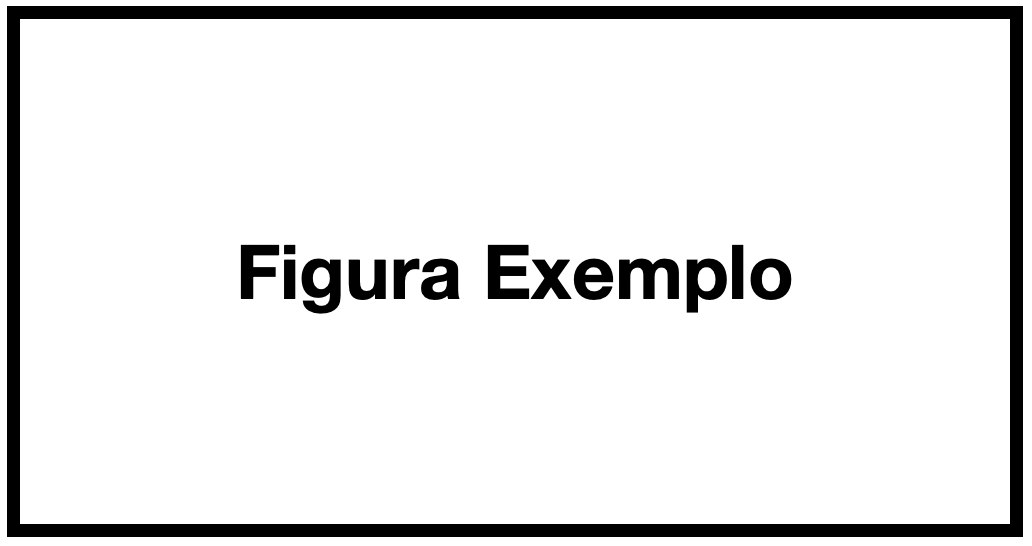
\includegraphics[width=.9\textwidth]{figura.png}
  \caption{Exemplo ilustrativo de figura.}
  \label{fig:exemplo}
\end{figure}

% ----------------------------------------------------------
\section{Considerações Finais}
As conclusões devem relacionar os resultados aos objetivos.  
Citação com página: \cite[p.~25]{azumaRecentAdvancesAugmentedReality2001}.

% ----------------------------------------------------------
\printbibliography

% ----------------------------------------------------------
\appendix
\renewcommand{\thesection}{Apêndice \Alph{section}}

\section{Exemplo de Apêndice}
Material complementar, questionários ou dados adicionais.

\end{document}